\documentclass[../main.tex]{subfiles}
\begin{document}


\section{Постановка краевых задач Дирихле и Неймана для уравнения Пуассона в ограниченной области. Единственность классического решения задачи Дирихле в классе $C^1(\overline{\Omega}) \cap C^2({\Omega})$. Неединственность решения задачи Неймана и необходимое условие её разрешимости.}
% Затехал Шлёнский Владос
\Subsection{Формулы Грина}
\begin{definition}
Ограниченная область $\Omega$ называется \textit{областью с гладкой границей}, если $\forall x_0 \in \Gamma = \partial \Omega$ найдутся:
\begin{itemize}
\item такая декартова СК , что начало в $x_0$, $\xi = (\xi_1, \ldots, \xi_n)$ -- координаты точек в этой СК
\item Окрестность $U_0(x^0) = \{\xi\colon |\xi^{'}| < r,\; |\xi_n| < h\}$, где $\xi^{'} = (\xi_1, \ldots, \xi_{n - 1})$, такая, что в $U_0(x^0)$ часть границы $\Gamma \cap U_0(x^0)$ представляется в виде: $\xi_n = F(\xi^{'}), \, |\xi^{'}| < r, \, F(0) = 0, \; F(\xi^{'}) \in C^1(|\xi^{'}| < r),\; \nabla_{\xi^{'}} F(0) = 0$, 
\item Множество $U_{-}(x^0) = U_0(x^0) \cap \{x\colon\; \xi_n < F(\xi^{'})\} \in \Omega$, \\
Множество $U_{+}(x^0) = U_0(x^0) \cap \{x\colon\; \xi_n \geq F(\xi^{'})\}\colon\; \Omega \cap U_{+} = \varnothing$
\item Числа $r > 0$, $h > 0$ можно выбрать независимо от $x^0 \in \Gamma$.
\end{itemize}
\end{definition}
\begin{minipage}{0.3\textwidth}
\begin{center}
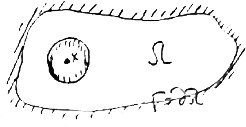
\includegraphics[scale = 0.2]{17_1_new}
\end{center}
\end{minipage}
\begin{minipage}{0.8\textwidth}
Для ограниченных областей с гладкими границами справедлива формула Остроградского-Гаусса ($F$ - непрерывно дифференцируемое векторное поле):
$$\int\limits_{\Omega} \div \vec{F}(x)\;dx = \int\limits_{\partial \Omega} \bigl(\vec{F}(x),\: \vec{n}\bigr)\;dS = \int\limits_{\Gamma} \bigl(\vec{F}(x),\: \vec{n}\bigr)\;dS$$
\end{minipage} \\
\begin{lemma} \ \\
\Subsubsection{Формулы Грина}
Пусть $\Omega$ -- ограниченная область с границей класса $C^1$ в $\R^n$, тогда справедливы следующие формулы.
	$$\forall u(x) \in C^2(\Omega)\cap C^1(\overline{\Omega}), v(x) \in C^1(\overline{\Omega}) \to \int\limits_{\Omega} (\Delta u)v\; dx = \oint\limits_{\Gamma} \dfrac{\partial u}{\partial \vec{n}} v\;dS_x - \int\limits_{\Omega}(\nabla u, \nabla v)\;dx $$
$$ \forall u(x), v(x) \in C^2(\overline{\Omega}) \to \int\limits_{\Omega} (\Delta u)v\; dx - \int\limits_{\Omega} (\Delta v)u\; dx = \oint\limits_{\Gamma} \dfrac{\partial u}{\partial \vec{n}} v\;dS_x - \oint\limits_{\Gamma} \dfrac{\partial v}{\partial \vec{n}} u\;dS_x$$
Полученные формулы называются первой и второй\; \textit{формулами Грина} соответственно.
\end{lemma}
\begin{proof}\ \\
\Subsubsection{Первая формула Грина}
Пусть $\vec{f}(x), v(x)$ - гладкие векторное и скалярное поля соответственно: $\div(\vec{f} \cdot v) = (\nabla, \overset{\shpos}{\vec{f}}v) + (\nabla, \vec{f}\overset{\shpos}{v}) = v\div \vec{f} + (\vec{f}, \grad{v})$. \\
Положим $\vec{f} = \nabla u \in C^1 \Rightarrow \div (v \nabla u) = v \underbrace{\div(\nabla u)}_{\Delta u} + (\nabla u, \nabla v)$. \\
Интегрируем по объёму в $\Omega$:
\begin{equation*}
	\int\limits_{\Omega} v \Delta u\;dx = 	\int\limits_{\Omega} \div(v\nabla u)\;dx -\int\limits_{\Omega} (\nabla u, \nabla v)\;dx = \oint\limits_{\Gamma}(v \nabla u, \vec{n})\;dS - \int\limits_{\Omega}(\nabla u, \nabla v)\;dx
\end{equation*}
Заметим, что:
$$(v\nabla u, \vec{n}) = v \sum\limits_{k = 1}^{\dim \R^n}\dfrac{\partial u(x)}{\partial x_k} n_k = \dfrac{\partial u}{\partial \vec{n}}(x) \cdot v(x)$$
При подстановке данного результата в равенство выше немедленно получим первую формулу Грина.
\Subsubsection{Вторая формула Грина}
Для получения второй формулы Грина необходимо вычесть из первой формулы Грина симметричное ему по $u$ и $v$ равенство:
$$\int\limits_{\Omega} u \Delta v\;dx = \oint\limits_{\Gamma}(u \nabla v, \vec{n})\;dS - \int\limits_{\Omega}(\nabla v, \nabla u)\;dx$$
\end{proof}

\Subsection{Внутрення задача Дирихе для уравнения Пуассона}
Пусть $\Omega$ -- ограниченная область с границей $\Gamma$ класса $C^1, u_0(x) \in C(\Gamma), f(x) \in C(\overline{\Omega})$. Требуется найти $u(x)$, удовлетворяющую условиям:
\begin{equation}
\label{eq:17_1}
	\begin{cases}
		\Delta u(x) = f(x), \quad x \in \Omega, \\
		u\bigr|_{\Gamma} = u_0(x).
	\end{cases}
\end{equation}
\textit{Классическим решением задачи Дирихле} (\ref{eq:17_1}) называется $u(x) \in C^1(\overline{\Omega}) \cap C^2({\Omega})$, удовлетворяющая уравнению и начальным условиям. \\
\begin{lemma}
Не может существовать более одного классического решения задачи (\ref{eq:17_1}).
\end{lemma}
\begin{proof}
Если $\exists u_{I}$ и $u_{II}$ - классические решения задачи (\ref{eq:17_1}), то $v(x) = u_{I} - u_{II}$ есть классическое решение полностью однородной задачи: $\Delta v \equiv 0,\; v\bigr|_{\Gamma} = 0$. \\
По формуле Грина:
\begin{equation*}
	\int\limits_{\Omega} v\cancelto{0}{\Delta v}\; dx = \oint\limits_{\partial \Omega}\dfrac{\partial v}{\partial \vec{n}}\cancelto{0}{v}\;dS - \int\limits_{\Omega}(\nabla v, \nabla v)\;dx \Rightarrow \nabla v \equiv 0 \Forall x \in \Omega \Rightarrow v(x) = \text{const}
\end{equation*}
С учётом того, что $\Delta v(x) = 0$ и $v(x)\bigr|_{\Gamma} = 0$, получим, что $v(x) = 0$, а значит, $u_{I} = u_{II}$, и решение единственно.
\end{proof}
\Subsection{Внутренняя задача Неймана для уравнения Пуассона}
Пусть $\Omega$ -- ограниченная область с границей класса $C^1, u_1(x) \in C(\Gamma), f(x) \in C(\overline{\Omega})$. Требуется найти $u(x)$ удовлетворяющую условиям:
\begin{equation}
\label{eq:17_2}
    \begin{cases}
        \Delta u(x) = f(x), & x \in \Omega, \\
	\dfrac{\partial u}{\partial \vec{n}} \biggr|_{\Gamma} = u_1(x).
    \end{cases}
\end{equation}
\begin{definition}
\textit{Классическое решение задачи Неймана} (\ref{eq:17_2}) есть такая функция $u(x) \in C^1(\overline{\Omega}) \cap C^2({\Omega})$, удовлетворяющая уравнению и граничным условиям.
\end{definition}
\begin{lemma}
Любые два классические решения задачи Неймана отличаются на константу.
\end{lemma}
\begin{proof}
Если $\exists u_{I}$ и $u_{II}$ - классические решения задачи (\ref{eq:17_2}), то $v(x) = u_{I} - u_{II}$ есть классическое решение полностью однородной задачи: $\Delta v \equiv 0,\; \dfrac{\partial v}{\partial \vec{n}}\bigr|_{\Gamma} = 0$. 
По формуле Грина имеем:
\begin{equation*}
 	\int\limits_{\Omega} v \cancelto{0}{\Delta v}\; dx = \oint\limits_{\Gamma} \cancelto{0}{\dfrac{\partial v}{\partial \vec{n}}}v\;dS - \int\limits_{\Omega} |\nabla v|^2\;dx \Rightarrow v \equiv \text{const}
\end{equation*}
\end{proof}
\begin{lemma}
Необходимым условием существования классического решения задачи Неймана является условие $\int\limits_{\Omega} f(x)\;dx = \oint\limits_{\Gamma}u_1(x)\;dS$.
\end{lemma}
\begin{proof}
\begin{equation*}
\int\limits_{\Omega} f(x)\;dx = \int\limits_{\Omega} \Delta u\;dx = \int\limits_{\Omega} \Delta u \cdot 1\; dx = \bigl[\text{1-ая ф. Грина}\bigr] = \int\limits_{\partial \Omega} \dfrac{\partial u}{\partial \vec{n}} \cdot 1\;dS - \cancelto{0}{\int\limits_{\Omega} (\nabla u, \nabla 1)\;dx} = \int\limits_{\partial \Omega} u_1(x) \;dS .
\end{equation*}
\end{proof}
\end{document}